

\documentclass{beamer}

\mode<presentation> {

% The Beamer class comes with a number of default slide themes
% which change the colors and layouts of slides. Below this is a list
% of all the themes, uncomment each in turn to see what they look like.


\usetheme{Boadilla}



\setbeamertemplate{footline}  


}
\setbeamersize{text margin left=1cm, }
\setbeamertemplate{frametitle}[default][center]
\usepackage{graphicx} 
\usepackage{booktabs} 

	\usepackage{changepage}


\usepackage{cite}
\usepackage{setspace}
\usepackage{color}
\usepackage[normalem]{ulem}
\newtheorem{hyp}{Hypothesis}


\usepackage{epsfig}
\usepackage{amsmath}
\usepackage{amssymb}
\usepackage{multicol}
\usepackage{amsmath, amsthm, amssymb}


\usepackage{graphicx}
\usepackage{tikz}
\usetikzlibrary{shapes,arrows}
\usepackage{tikz}
\usepackage{amsmath, amsthm, amssymb}
%----------------------------------------------------------------------------------------
%	TITLE PAGE
%----------------------------------------------------------------------------------------



\begin{document}
	

  

\begin{frame}
	\frametitle{Unsupervised Models}
	\begin{itemize}
		\item An unusual place to begin \pause 
		\item Most data science classes focus on supervised models \pause 
		\item Partially practicality \pause 
		\item Unsupervised models: the past and future of data
	\end{itemize} 
\end{frame}




\begin{frame}
	\frametitle{Unsupervised Models -- Yann LeCunn}
	 
	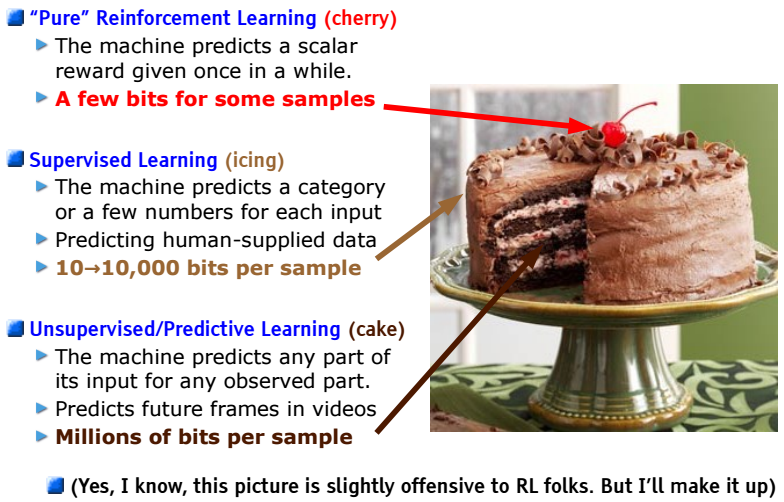
\includegraphics[ scale=.4]{figures/lecunn_icing.png} \\
\end{frame}







\begin{frame}
	\frametitle{Quantities for comparing texts}
	\begin{description}
		\item[Length] in characters, words, lines, sentences, paragraphs,
		pages, sections, chapters, etc.
		\item[Readability statistics]  Use a combination of syllables and
		sentence length to indicate ``readability'' in terms of complexity
		\item[Vocabulary diversity] (At its simplest) involves measuring a
		\emph{type-to-token ratio} (TTR) where unique words are types and
		the total words are tokens
		\item[Word (relative) frequency] counts or proportions of words
		
	\end{description}
\end{frame}


% \begin{frame}
%  \frametitle{Simple descriptive table about texts: Describe your data!}
%  \scriptsize
%  \centering
%  \begin{tabular}{llrr}
%   \hline
%   Speaker               & Party & Tokens &
%   Types	\\
%   \hline\hline
%   Brian	Cowen           & FF    & 5,842  & 1,466 \\
%   Brian	Lenihan         & FF    & 7,737  & 1,644 \\
%   Ciaran	Cuffe          & Green & 1,141  & 421   \\
%   John	Gormley	(Edited) & Green & 919    & 361   \\
%   John	Gormley (Full)   & Green & 2,998  & 868   \\
%   Eamon	Ryan            & Green & 1,513  & 481   \\
%   Richard	Bruton        & FG    & 4,043  & 947   \\
%   Enda	Kenny            & FG    & 3,863  & 1,055 \\
%   Kieran	ODonnell       & FG    & 2,054  & 609   \\
%   Joan	Burton           & LAB   & 5,728  & 1,471 \\
%   Eamon	Gilmore         & LAB   & 3,780  & 1,082 \\
%   Michael	Higgins       & LAB   & 1,139  & 437   \\
%   Ruairi	Quinn          & LAB   & 1,182  & 413   \\
%   Arthur	Morgan         & SF    & 6,448  & 1,452 \\
%   Caoimhghin	O'Caolain  & SF    & 3,629  &
%   1,035 	\\[1ex]
%   All Texts             &       & 49,019 & 4,840 \\[1ex]
%   \multicolumn{2}{l}{\emph{Min}}	&	 919 	&	 361 	\\
%   \multicolumn{2}{l}{\emph{Max}}	&	 7,737 	&	 1,644 	\\
%   \multicolumn{2}{l}{\emph{Median}}	&	 3,704 	&	 991 \\
%   \multicolumn{2}{l}{\em Hapaxes with Gormley Edited} & 67                 \\
%   \multicolumn{2}{l}{\em Hapaxes with Gormley Full Speech} & 69                 \\
%   \hline
%  \end{tabular}
%
% \end{frame}



\begin{frame}
	\frametitle{Lexical Diversity}
	\begin{itemize}
		\item Basic measure is the \alert{TTR}: Type-to-Token ratio
		\item Problem: This is very sensitive to overall document length, as
		shorter texts may exhibit fewer word repetitions
		\item Special problem: length may relate to the introdution of
		additional subjects, which will also increase richness
	\end{itemize}
\end{frame}



\begin{frame}
	\frametitle{Complexity and Readability}
	\begin{itemize}
		\item Use a combination of syllables and sentence length to indicate
		``readability'' in terms of complexity
		\item Common in educational research, but could also be used to
		describe textual complexity
		\item Most use some sort of sample
		\item No natural scale, so most are calibrated in terms of some
		interpretable metric
		\item Implemented in \textbf{quanteda} as \texttt{textstat\_readability()}
	\end{itemize}
\end{frame}


\begin{frame}
	\frametitle{Flesch-Kincaid readability index}
	\begin{itemize}
		\item F-K is a modification of the original \alert{Flesch Reading Ease Index}:
		\begin{equation*}
		206.835 - 1.015 \left( \frac{\mathrm{total\ words}}{\mathrm{total\
				sentences}} \right) - 84.6 \left( \frac{\mathrm{total\ syllables}}{\mathrm{total\
				words}} \right)
		\end{equation*}
		{\color{blue} Interpretation:} 0-30: university level; 60-70:
		understandable by 13-15 year olds; and 90-100 easily understood by
		an 11-year old student.
		\item \pause \alert{Flesch-Kincaid} rescales to the US educational grade
		levels (1--12):
		\begin{equation*}
		0.39 \left( \frac{\mathrm{total\ words}}{\mathrm{total\
				sentences}} \right) + 11.8 \left( \frac{\mathrm{total\ syllables}}{\mathrm{total\
				words}} \right) - 15.59
		\end{equation*}
	\end{itemize}
\end{frame}

\begin{frame}
	\frametitle{Documents as vectors}
	\begin{itemize}
		\item The idea is that (weighted) features form a vector for each
		document, and that these vectors can be judged using metrics of \alert{similarity}
		\item A document's vector for us is simply (for us) the row of the
		document-feature matrix
	\end{itemize}
\end{frame}


\begin{frame}
	\frametitle{Characteristics of similarity measures}
	Let $A$ and $B$ be any two documents in a set and $d(A,B)$ be the distance between $A$ and $B$.
	\begin{enumerate}
		\item \alert{$d(x, y) \geq 0$} (the distance between any two points
		must be non-negative)
		\item \alert{$d(A, B) = 0$ iff $A = B$} (the distance between two
		documents must be zero if and only if the two objects are
		identical)
		\item \alert{$d(A, B) = d(B, A)$} (distance must be symmetric: $A$ to
		$B$ is the same distance as from $B$ to $A$)
		\item \alert{$d(A, C) \leq d(A, B) + d(B, C)$} (the measure must satisfy the triangle inequality)
	\end{enumerate}
\end{frame}

\begin{frame}
	\frametitle{Euclidean distance}
	Between document $A$ and $B$ where $j$ indexes their features, where
	$y_{ij}$ is the value for feature $j$ of document $i$
	\begin{itemize}
		\item Euclidean distance is based on the Pythagorean theorem
		\item Formula
		\begin{equation}
		\sqrt{\sum_{j=1}^j (y_{Aj} - y_{Bj})^2}
		\end{equation}
		\item In vector notation:
		\begin{equation}
		\| \mathbf{y}_{A} - \mathbf{y}_{B} \|
		\end{equation}
		\item Can be performed for any number of features $J$ (or $V$ as the
		vocabulary size is sometimes called -- the number of columns in of
		the dfm, same as the number of feature types in the corpus)
	\end{itemize}
\end{frame}


\begin{frame}
	\frametitle{A geometric interpretation of ``distance''}
	In a right angled triangle, the cosine of an angle $\theta$ or
	$\mathsf{cos}(\theta)$ is the \alert{length of the adjacent side}
	divided by the \alert{length of the hypotenuse}
	\begin{center}
		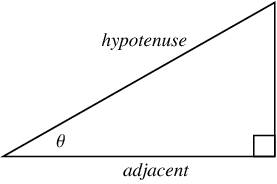
\includegraphics[width=6cm]{figures/cosine.png}
	\end{center}
	
	We can use the vectors to represent the text location in a
	$V$-dimensional vector space and compute the angles between them
\end{frame}



\begin{frame}
	\frametitle{Cosine similarity}
	\begin{itemize}
		\item Cosine distance is based on the size of the angle between the vectors
		\item Formula
		\begin{equation}
		\frac{\mathbf{y}_{A} \cdot \mathbf{y}_{B}}{\| \mathbf{y}_{A}\| \| \mathbf{y}_{B}\| }
		\end{equation}
		\item The $\cdot$ operator is the dot product, or $\sum_{j}
		y_{Aj}y_{Bj}$
		\item The $\| \mathbf{y}_{A}\|$ is the vector norm of the (vector
		of) features vector $\mathbf{y}$
		for document $A$, such that $\| \mathbf{y}_{A}\| = \sqrt{\sum_j y_{Aj}^2}$
		\item \pause Nice property: independent of document length, because it
		deals only with the angle of the vectors
		\item Ranges from -1.0 to 1.0 for term frequencies, or 0 to 1.0 for
		normalized term frequencies (or tf-idf)
	\end{itemize}
\end{frame}

\begin{frame}
	\frametitle{Cosine similarity illustrated}
	\begin{center}
		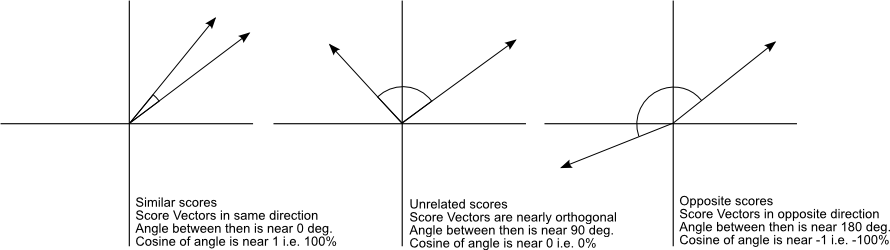
\includegraphics[width=11cm]{figures/cosinesimilarity.png}
	\end{center}
\end{frame}

\begin{frame}
	\frametitle{Example text}
	\begin{center}
		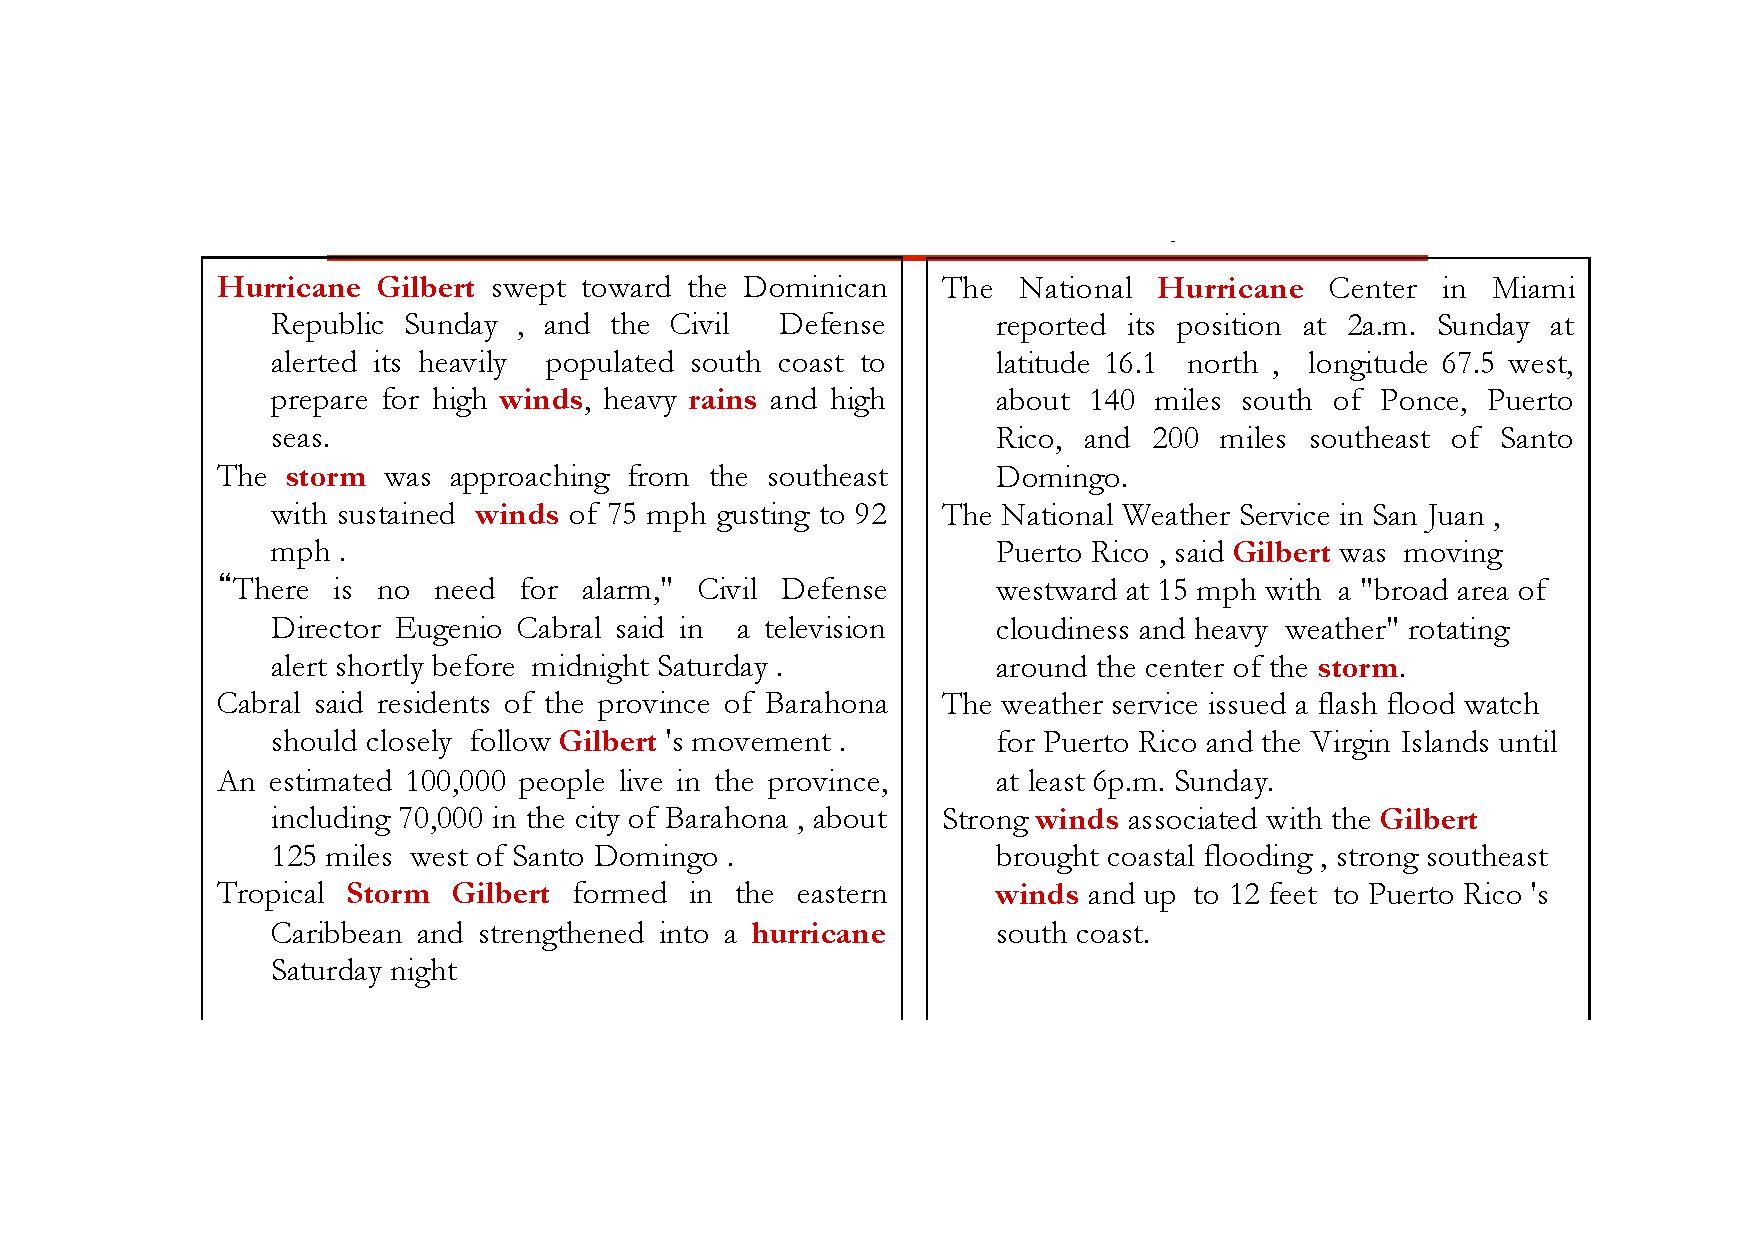
\includegraphics[width=11cm]{figures/gilbertdocs.pdf}
	\end{center}
\end{frame}

\begin{frame}
	\frametitle{Example text: selected terms}
	\begin{itemize}
		\item \alert{Document 1} \newline Gilbert: 3, hurricane: 2, rains: 1, storm: 2,
		winds: 2 \newline
		\item \alert{Document 2} \newline Gilbert: 2, hurricane: 1, rains: 0, storm: 1,
		winds: 2
	\end{itemize}
\end{frame}

\begin{frame}[fragile]
	\frametitle{Example text: cosine similarity in R}
	\begin{center}
		\begin{footnotesize}
			\begin{verbatim}
			toyDfm <- as.dfm(matrix(c(3,2,1,2,2, 2,1,0,1,2),
			nrow = 2, byrow = TRUE))
			colnames(toyDfm) <- c("Gilbert", "hurricane", "rain", "storm", "winds")
			toyDfm
			## Document-feature matrix of: 2 documents, 5 features (10% sparse).
			## 2 x 5 sparse Matrix of class "dfm"
			##        features
			## docs    Gilbert hurricane rain storm winds
			##   text1       3         2    1     2     2
			##   text2       2         1    0     1     2
			
			textstat_simil(toyDfm, method = "cosine")
			##           text1
			## text2 0.9438798
			\end{verbatim}
		\end{footnotesize}
	\end{center}
\end{frame}


\begin{frame}
	\frametitle{Relationship to Euclidean distance}
	\begin{itemize}
		\item Cosine similarity measures the similarity of vectors with
		respect to the origin
		\item Euclidean distance measures the distance between particular
		points of interest along the vector
		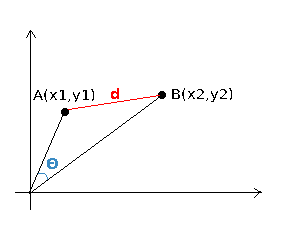
\includegraphics[width=.5\textwidth]{figures/cosineVEuclid.png}
	\end{itemize}
\end{frame}


% \begin{frame}
%   \frametitle{Relationship to Euclidean distance}
%   \begin{itemize}
%   \item Euclidean distance is $\| \mathbf{y}_{A} - \mathbf{y}_{B} \|$
%   \item $\mathsf{cos}(A, B) = \frac{\mathbf{y}_{A} \cdot
%       \mathbf{y}_{B}}{\| \mathbf{y}_{A}\| \| \mathbf{y}_{B}\|
%     }$
%   \end{itemize}
%   If $A$ and $B$ are normalized to unit length (term proportions
%   instead of frequencies), such that $\|A\|^2 = \|B\|^2 = 1$, then
%   \begin{eqnarray}
%     \| \mathbf{y}_{A} - \mathbf{y}_{B} \|^2 &=& (A - B)'(A-B) \nonumber
% \\
% &=& \|A\|^2 + \|B\|^2 - 2~A'B \nonumber \\
% &=& 2(1 - cos(A, B)) \nonumber
%   \end{eqnarray}
% where $(1 - cos(A, B))$ is the complement of the cosine similarity,
% also known as \emph{cosine distance} \newline \vspace{.5ex}

% so the Euclidean distance is twice the cosine distance for normalized
% term vectors
% \end{frame}


\begin{frame}
	\frametitle{Jacquard coefficient}
	\begin{itemize}
		\item Similar to the Cosine similarity
		\item Formula
		\begin{equation}
		\frac{\mathbf{y}_{A} \cdot \mathbf{y}_{B}}{\| \mathbf{y}_{A}\|
			+ \| \mathbf{y}_{B}\|  - \mathbf{y}_{A} \cdot \mathbf{y}_{B}}
		\end{equation}
		\item Ranges from 0 to 1.0
		%\item The $\times$ operator is a ????
	\end{itemize}
\end{frame}

\begin{frame}
	\frametitle{Example: Inaugural speeches}
	\begin{center}
		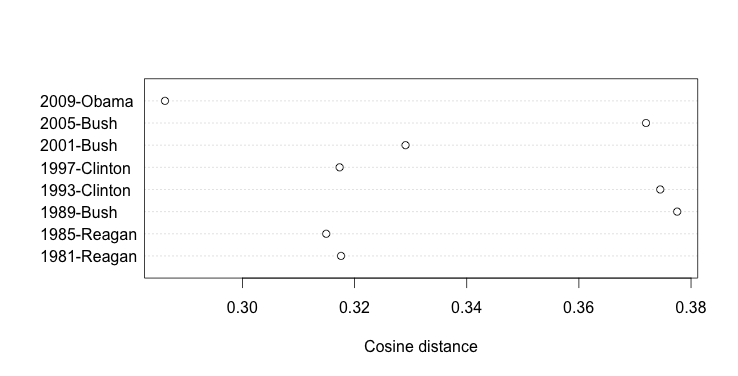
\includegraphics[width=.9\textwidth]{figures/prescosinedist.png}
	\end{center}
\end{frame}

\begin{frame}
	\frametitle{Example: Inaugural speeches}
	\begin{center}
		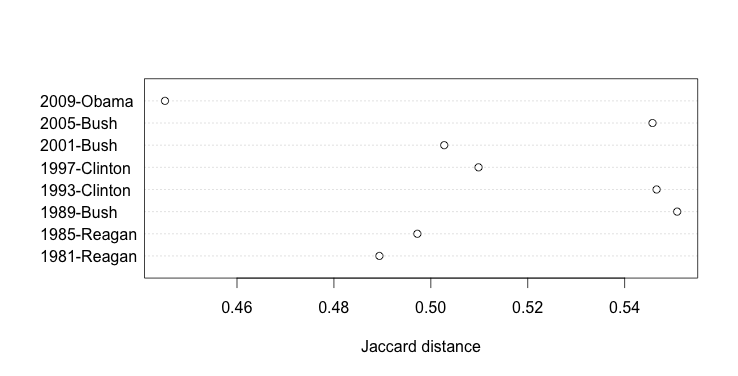
\includegraphics[width=.9\textwidth]{figures/presjaccarddist.png}
	\end{center}
\end{frame}




\begin{frame}
	\frametitle{Typical features}
	\begin{itemize}
		\item Normalized term frequency (almost certainly)
		\item Very common to use tf-idf -- if not, similarity is boosted
		by common words (stop words)
		\item Not as common to use binary features
	\end{itemize}
	
\end{frame}














\begin{frame}
	\frametitle{Weighting strategies for feature counting}
	\begin{description}
		\item[term frequency] Some approaches trim very low-frequency words.
		Rationale: get rid of rare words that expand the feature matrix
		but matter little to substantive analysis
		\item[document frequency] Could eliminate words appearing in few documents
		\item[inverse document frequency] Conversely, could weight words
		more that appear in the most documents
		\item[\emph{tf-idf}] a combination of term frequency and inverse
		document frequency, common method for feature weighting
	\end{description}
\end{frame}

\begin{frame}
	\frametitle{Strategies for feature \emph{weighting}: tf-idf}
	\begin{itemize}
		\setlength{\itemsep}{3ex}
		\item $tf_{i,j} = \frac{n_{i,j}}{\sum_kn_{k,j}}$
		where $n_{i,j}$ is number of occurences of term $t_i$ in document
		$d_j$, $k$ is total number of terms in document $d_j$
		\item $idf_i = \mathrm{ln} \frac{|D|}{|\left\{ d_j: t_i \in d_j \right\} |}$
		
		where
		\begin{itemize}
			\item $|D|$ is the total number of documents in the set
			\item $|\left\{ d_j: t_i \in d_j \right\} |$ is the number of
			documents where the term $t_i$ appears (i.e. $n_{i,j}\neq 0$)
		\end{itemize}
		
		\item \emph{tf-idf}$_i = \mathit{tf}_{i,j} \cdot \mathit{idf}_i$
	\end{itemize}
\end{frame}

\begin{frame}
	\frametitle{Computation of tf-idf: Example}
	Example: We have 100 political party manifestos, each with 1000
	words.  The first document contains 16 instances of the word
	``environment''; 40 of the manifestos contain the word
	``environment''.
	\vspace{2ex}
	\begin{itemize}
		\setlength{\itemsep}{1.2ex}
		\item The \emph{term frequency} is $16/1000 = 0.016$
		\item The \emph{document frequency} is $100/40 = 2.5$, or
		ln$(2.5)=0.916$
		\item The \emph{tf-idf} will then be $0.016 * 0.916 = 0.0147$
		\item \pause If the word had only appeared in 15 of the 100 manifestos,
		then the \emph{tf-idf} would be 0.0304 (three times higher).
		\item \pause A high weight in tf-idf is reached by a high term frequency
		(in the given document) and a low document frequency of the term
		in the whole collection of documents; hence the \alert{weights hence tend to
			filter out common terms}
	\end{itemize}
\end{frame}



\begin{frame}
	\frametitle{The idea of "clusters"}
	\begin{itemize}
		\item Essentially: groups of items such that inside a cluster they
		are very similar to each other, but very different from those
		outside the cluster
		\item ``unsupervised classification'': cluster is not to relate
		features to classes or latent traits, but rather to estimate
		membership of distinct groups
		\pause \item groups are given labels through post-estimation interpretation
		of their elements
		\item typically used when we do not and never will know the ``true''
		class labels
		\item issues: how to weight distance is arbitrary
		\begin{itemize}
			\pause \item which dimensionality? (determined by which
			features are selected)
			\pause \item how to weight distance is arbitrary
			\pause \item different metrics for distance
		\end{itemize}
	\end{itemize}
\end{frame}


\begin{frame}
	\frametitle{$k$-means clustering}
	\begin{itemize}
		\item Essence: assign each item to one of $k$ clusters, where the
		goal is to minimised within-cluster difference and maximize
		between-cluster differences
		\item Uses random starting positions and iterates until stable
		\item as with $kNN$, $k$-means clustering treats feature values as
		coordinates in a multi-dimensional space
		\item \pause Advantages
		\begin{itemize}
			\item simplicity
			\item highly flexible
			\item efficient
		\end{itemize}
		\item \pause Disadvantages
		\begin{itemize}
			\item no fixed rules for determining $k$
			\item uses an element of randomness for starting values
		\end{itemize}
	\end{itemize}
\end{frame}

\begin{frame}
	\frametitle{algorithm details}
	\begin{enumerate}
		\item \pause Choose starting values
		\begin{itemize}
			\item \pause assign random positions to $k$ starting values that will
			serve as the ``cluster centres'', known as ``centroids'' ; or,
			\item assign each feature randomly to one of $k$ classes
		\end{itemize}
		\item \pause assign each item to the class of the centroid that is ``closest''
		\begin{itemize}
			\item Euclidean distance is most common
			\item any others may also be used (Manhattan, Minkowski,
			Mahalanobis, etc.)
			\item (assumes feature vectors have been normalised within item)
		\end{itemize}
		\item  \pause update: recompute the cluster centroids as the mean value of
		the points assigned to that cluster
		\item  \pause repeat reassignment of points and updating centroids
		\item  \pause repeat 2--4 until some stopping condition is satisfied
		\begin{itemize}
			\item e.g.\@ when no items are reclassified following update of centroids
		\end{itemize}
		
	\end{enumerate}
\end{frame}

\begin{frame}
	\frametitle{$k$-means clustering illustrated}
	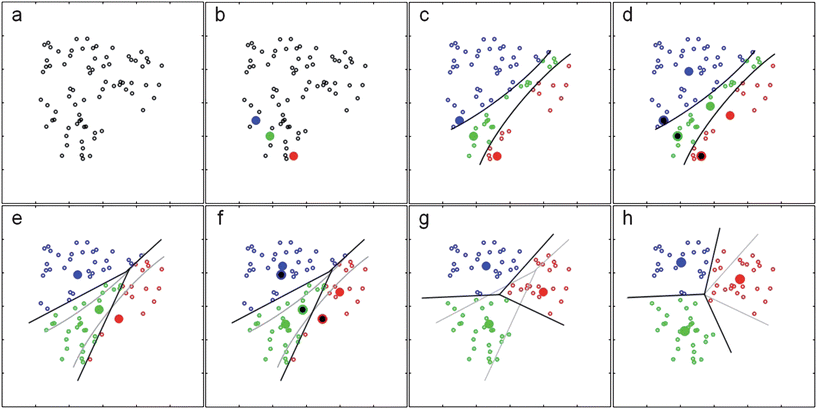
\includegraphics[width=\textwidth]{figures/kmeans.png}
\end{frame}

\begin{frame}
	\frametitle{choosing the appropriate number of clusters}
	\begin{itemize}
		\item very often based on prior information about the number of
		categories sought
		\begin{itemize}
			\item for example, you need to cluster people in a class into a
			fixed number of (like-minded) tutorial groups
		\end{itemize}
		\item a (rough!) guideline: set $k = \sqrt{N/2}$ where $N$ is the
		number of items to be classified
		\begin{itemize}
			\item usually too big: setting $k$ to large values will improve within-cluster
			similarity, but risks \emph{overfitting}
		\end{itemize}
	\end{itemize}
\end{frame}

\begin{frame}
	\frametitle{choosing the appropriate number of clusters}
	\begin{itemize}
		\item ``elbow plots'': fit multiple clusters with different $k$
		values, and choose $k$ beyond which are diminishing gains
		\vspace*{3ex}
		
		\hspace*{-1.4cm}
		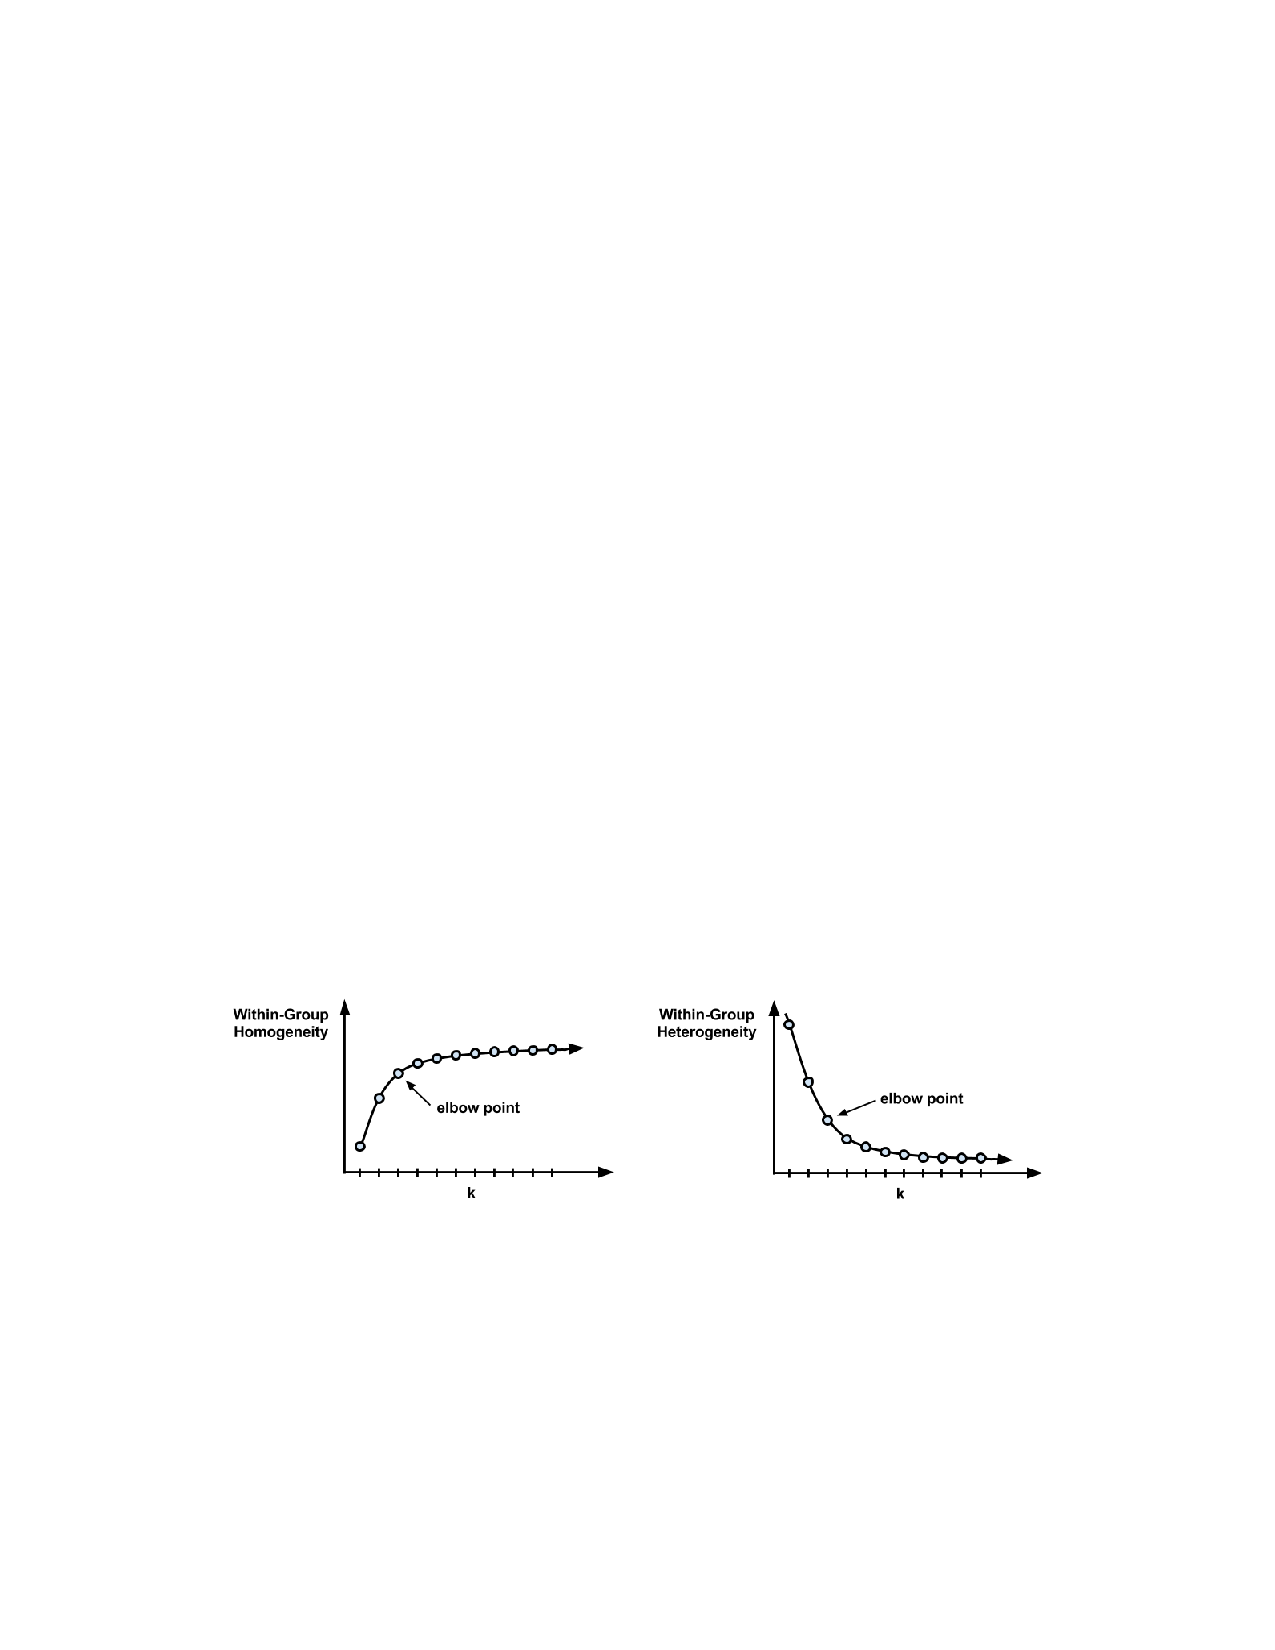
\includegraphics[width=1.1\textwidth]{figures/elbowplots.pdf}
	\end{itemize}
\end{frame}

\begin{frame}
	\frametitle{choosing the appropriate number of clusters}
	\begin{itemize}
		\item ``fit'' statistics to measure homogeneity within clusters and
		heterogeneity in between
		\item Entropy
		\item Perplexity
		\end{itemize}
	
\end{frame}

\begin{frame}
	\frametitle{Other clustering methods: hierarchical clustering}
	\begin{itemize}
		\item \emph{agglomerative}: works from the bottom up to create clusters
		\item \pause  like $k$-means, usually involves \emph{projection}: reducing
		the features through either selection or projection to a
		lower-dimensional representation
		\begin{enumerate}
			\item local projection: reducing features within document
			\item global projection: reducing features across all documents (Sch\"utze and Silverstein, 1997)
			\item \pause SVD methods, such PCA on a normalised feature matrix
			\item usually simple threshold-based truncation is used \newline (keep all
			but 100 highest frequency or tf-idf terms)
		\end{enumerate}
		\item \pause frequently/always involves weighting (normalising term
		frequency, tf-idf)
	\end{itemize}
\end{frame}

\begin{frame}
	\frametitle{hierarchical clustering algorithm}
	\begin{enumerate}
		\item start by considering each item as its own cluster, for $n$ clusters
		\item \pause calculate the $N(N-1)/2$ pairwise distances between each of
		the $n$ clusters, store in a matrix $D_0$
		\item \pause find smallest (off-diagonal) distance in $D_0$, and merge the
		items corresponding to the $i, j$ indexes in $D_0$ into a new ``cluster''
		\item \pause recalculate distance matrix $D_1$ with new cluster(s).
		\pause options for determining the location of a cluster include:
		\begin{itemize}
			\item centroids (mean)
			\item most dissimilar objects
			\item Ward's measure(s) based on minimising variance
		\end{itemize}
		\item \pause repeat 3--4 until a stopping condition is reached
		\begin{itemize}
			\item e.g.\@ all items have been merged into a single cluster
		\end{itemize}
		\item \pause to plot the \emph{dendrograms}, need decisions on ordering, since
		there are $2^{(N-1)}$ possible orderings
	\end{enumerate}
\end{frame}


\begin{frame}
	\frametitle{Dendrogram: Presidential State of the Union addresses}
	\hspace*{-1cm}
	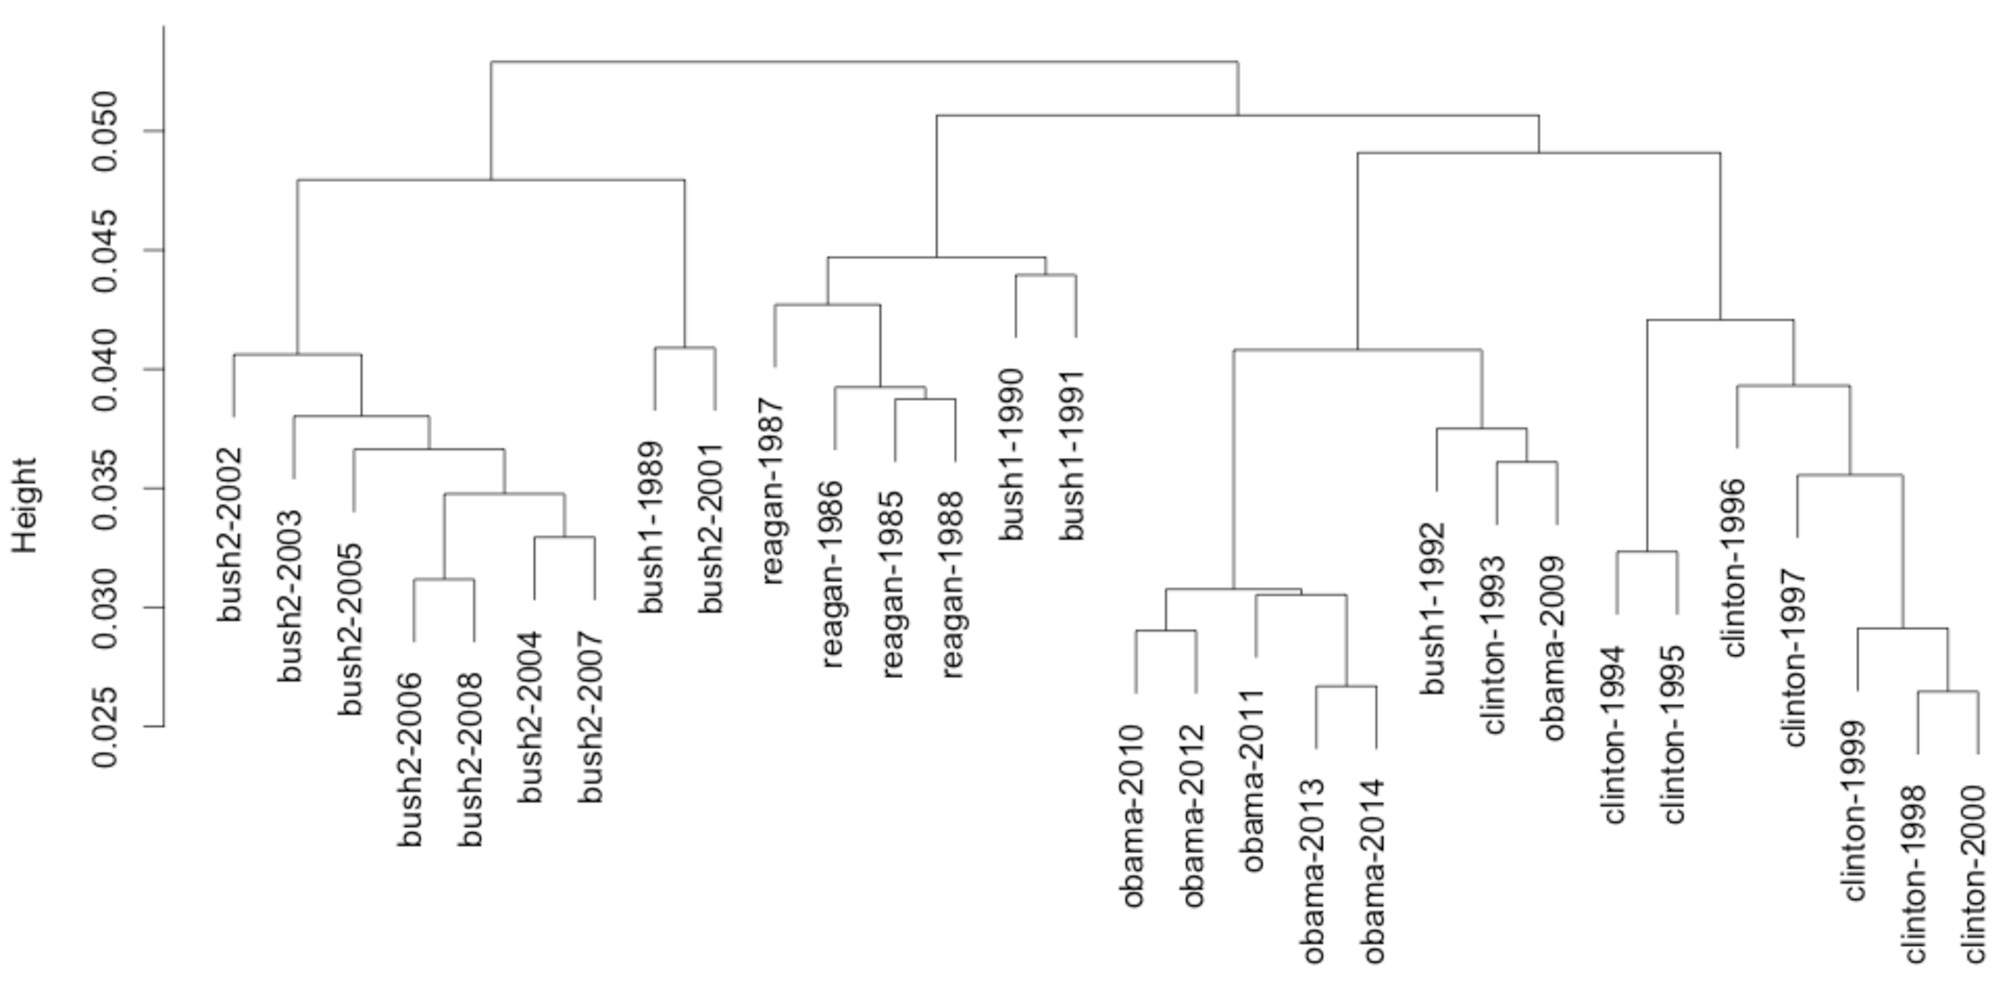
\includegraphics[width=1.15\textwidth]{figures/speechDendrogram.pdf}
\end{frame}


\begin{frame}
	\frametitle{Dendrogram: Presidential State of the Union addresses}
	\hspace*{-1cm}
	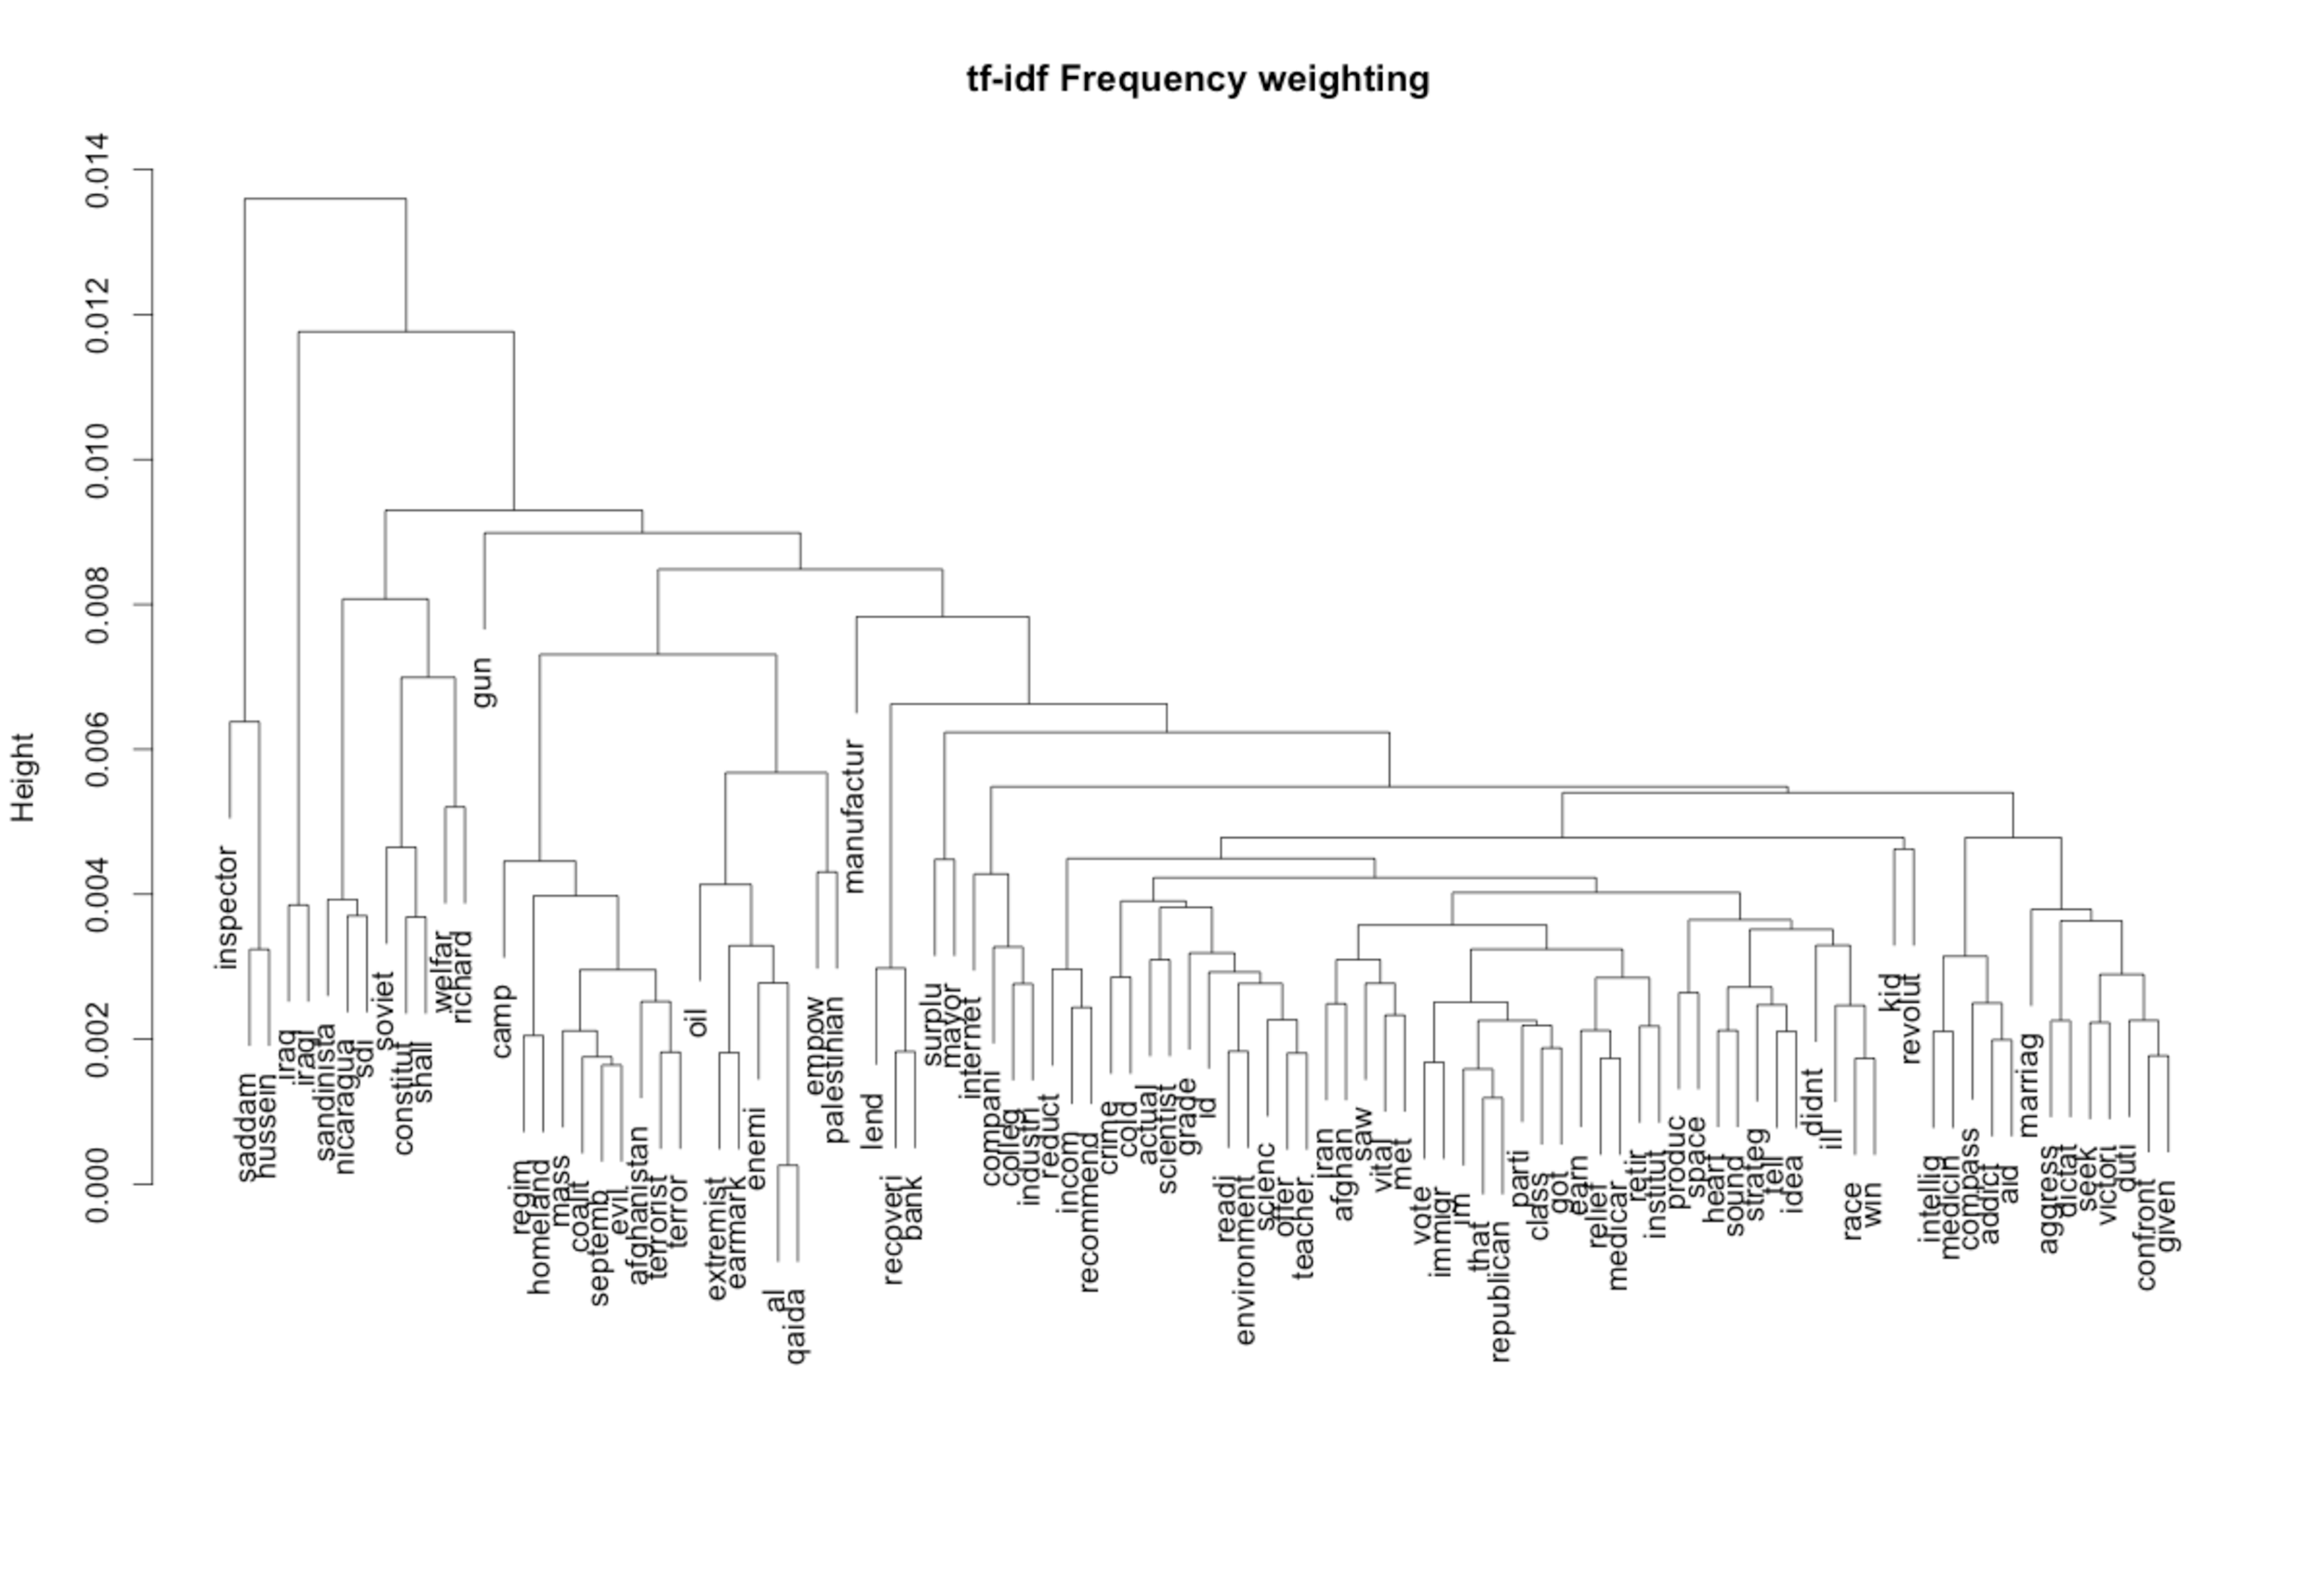
\includegraphics[width=1.15\textwidth]{figures/dendrogram1.pdf}
\end{frame}

\begin{frame}
	\frametitle{pros and cons of hierarchical clustering}
	\begin{itemize}
		\item advantages
		\begin{itemize}
			\item deterministic, unlike $k$-means
			\item no need to decide on $k$ in advance (although can specify as
			a stopping condition)
			\item allows hierarchical relations to be examined \newline (usually
			through \emph{dendrograms})
		\end{itemize}
		\item \pause disadvantages
		\begin{itemize}
			\item more complex to compute: quadratic in complexity: $O(n^2)$
			\newline -- whereas $k$-means has complexity that is $O(n)$
			\item the decision about where to create branches and in what
			order can be somewhat arbitrary, determined by method of
			declaring the ``distance'' to already formed clusters
			\item for words, tends to identify collocations as base-level
			clusters (e.g. ``saddam'' and ``hussein'')
		\end{itemize}
	\end{itemize}
\end{frame}

\begin{frame}
	\frametitle{Dendrogram: Presidential State of the Union addresses}
	\begin{center}
		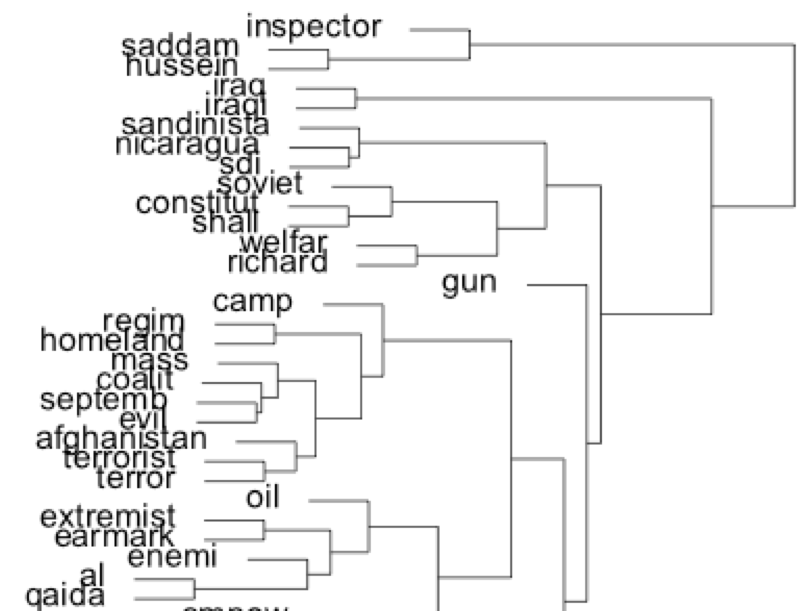
\includegraphics[height=7cm]{figures/dendrogram2.png}
	\end{center}
\end{frame}


\begin{frame}
	\frametitle{Topic Models}
	\begin{itemize}
		\item Topic models are algorithms for discovering the main
		``themes'' in an unstructured corpus
		\item Requires no prior information, training set, or special
		annotation of the texts \newline -- only a decision on $K$ (number of topics)
		\item A probabilistic, generative advance on several earlier
		methods, ``Latent Semantic Analysis'' (LSA) and ``probabilistic latent
		semantic indexing'' (pLSI)
	\end{itemize}
\end{frame}








\begin{frame}
	\frametitle{Unsupervised methods scale \alert{distance}}
	\begin{itemize}[<+->]
		\item Text gets converted into a quantitative matrix of
		\alert{features}
		\begin{itemize}
			\item words, typically
			\item could be dictionary entries, or parts of speech
		\end{itemize}
		\item Documents are scaled based on similarity/distance in feature use
		\item Fundamental problem: \alert{distance on which scale?}
		\begin{itemize}
			\item Ideally, something we care about, e.g. policy positions, ideology, preferences, sentiment
			\item But often other dimensions (language, rhetoric style, authorship) are more predictive
		\end{itemize}
		\item First dimension in unsupervised scaling will capture main source of variation, whatever that is
		\item Unlike supervised models, validation comes \alert{after} estimating the model
	\end{itemize}
\end{frame}



\begin{frame}
	\frametitle{Correspondence Analysis}  
	\begin{itemize}
		\item CA is like factor analysis for categorical data
		\item Following normalization of the marginals, it uses Singular
		Value Decomposition to reduce the dimensionality of the
		document-feature matrix
		\item This allows projection of the positioning of the words as well
		as the texts into multi-dimensional space
		\item The number of dimensions -- as in factor analysis -- can be
		decided based on the eigenvalues from the SVD
	\end{itemize}
\end{frame}

\begin{frame}
	\frametitle{Singular Value Decomposition}  
	\begin{itemize}
		\item A matrix $\underset{n\times
			k}{\mathbf{X}}$ can be represented in a dimensionality equal to its
		rank $d$ as:
		\begin{align}
		\underset{n\times k}{\mathbf{X}} &= \underset{n\times d}{\mathbf{U}}
		\ 
		\underset{d\times d}{\mathbf{\Sigma}} \ \underset{d\times k}{\mathbf{V}'}
		\end{align}
		\item The \textbf{U}, $\mathbf{\Sigma}$, and \textbf{V} matrixes ``relocate''
		the elements of $\mathbf{X}$ onto new coordinate vectors in
		$d$-dimensional Euclidean space
		\item Row variables of \textbf{X} become points on the \textbf{U}
		column coordinates, and the column variables of \textbf{X} become
		points on the \textbf{V} column coordinates
		\item The coordinate vectors are perpendicular (\emph{orthogonal}) to
		each other and are normalized to unit length
	\end{itemize}
\end{frame}

\begin{frame}
	\frametitle{Correspondence analysis}
	
	\begin{enumerate}[<+->]
		\item Compute matrix of standardized residuals, $\mathbf{S}$:\\
		\vspace{-.8cm}
		\begin{align*}\mathbf{S} = \mathbf{D}_r^{1/2} (\mathbf{P}-\mathbf{rc}^{T})\mathbf{D}_c^{1/2} \end{align*}\\
		\vspace{-.3cm}
		\begin{tabular}{ll}
			where & $\mathbf{P}=\mathbf{Y}/\sum_{ij}y_{ij}$\\
			&$\mathbf{r}$, $\mathbf{c}$ are row/column masses: e.g. $r_i=\sum_j p_{ij}$\\
			&$\mathbf{D}_r=\textrm{diag}(\mathbf{r})$, $\mathbf{D}_c=\textrm{diag}(\mathbf{c})$
		\end{tabular}
		\vspace{.25cm}
		\item Calculate SVD of $\mathbf{S}$
		\vspace{.25cm}
		\item Project rows and columns onto low-dimensional space:\\
		\vspace{-.8cm}
		\begin{align*}
		\mathbf{\theta}=\mathbf{D}_r^{1/2} \mathbf{U} & \textrm{ for rows (documents)}\\
		\vspace{-.2cm}
		\mathbf{\phi}=\mathbf{D}_c^{1/2} \mathbf{V} &  \textrm{ for columns (words)}
		\end{align*}
		\item[] Mathematically close to \alert{log-linear poisson regression model} {\color{gray}\footnotesize{(Lowe, 2008)}}
	\end{enumerate}
\end{frame}

\begin{frame}
	\frametitle{Example: Schonhardt-Bailey (2008) - speakers}
	\begin{center}
		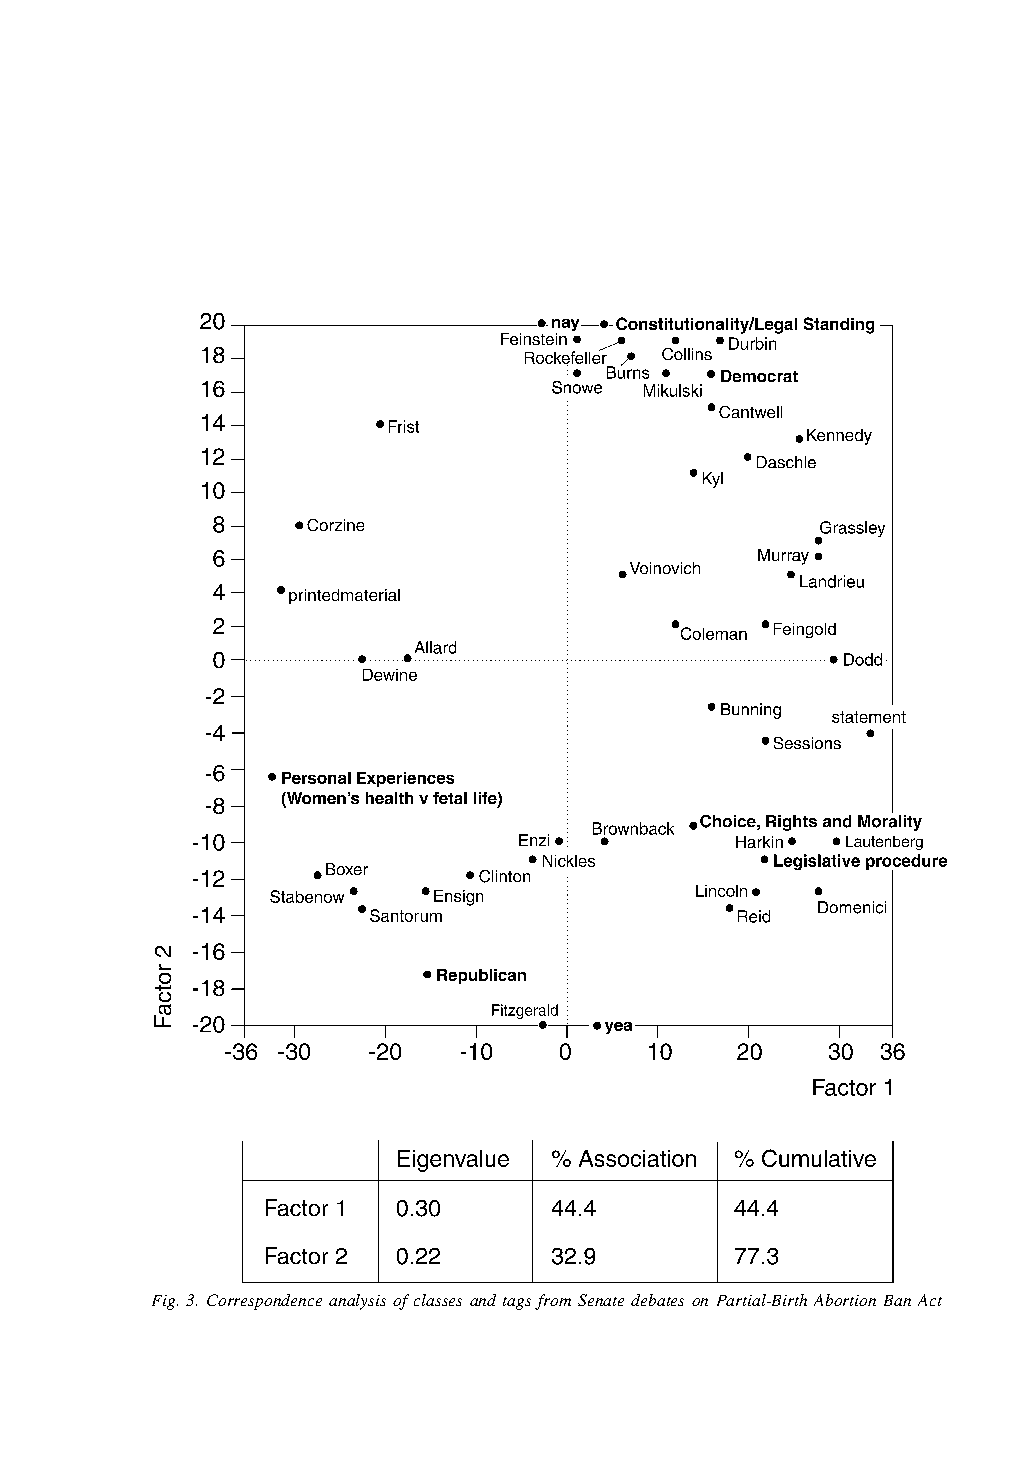
\includegraphics[width=6.7cm]{figures/SBca.pdf}
	\end{center}
\end{frame}

\begin{frame}
	\frametitle{Example: Schonhardt-Bailey (2008) - words}
	\begin{center}
		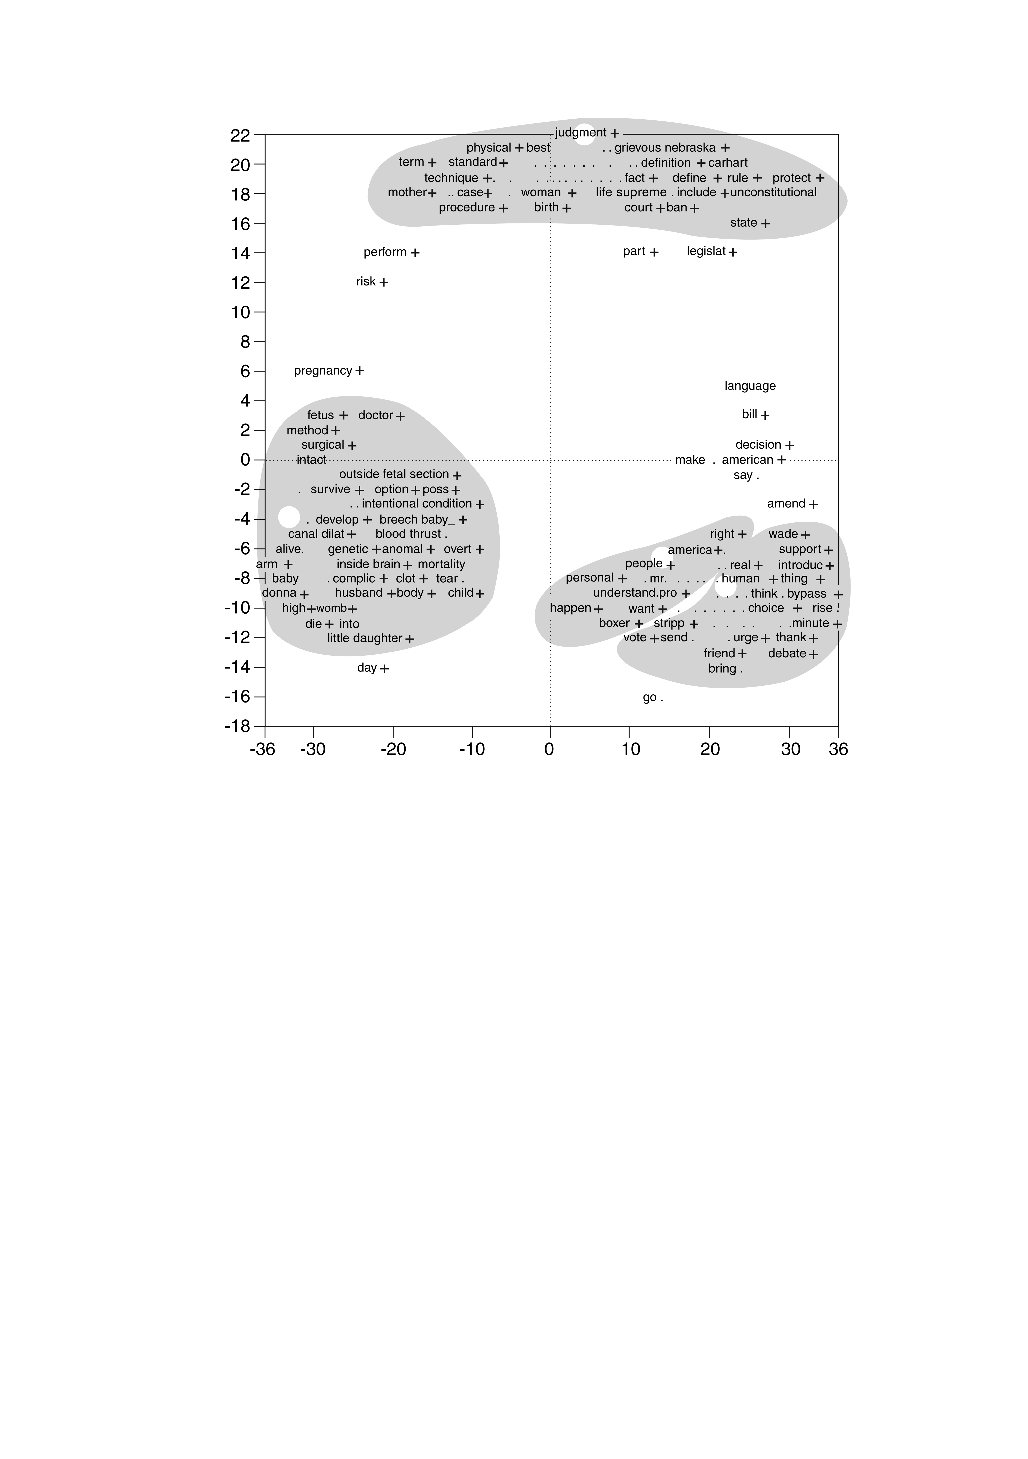
\includegraphics[width=8cm]{figures/SBca2.pdf}
	\end{center}
\end{frame}


\begin{frame}
	\frametitle{Interpreting scaled dimensions}
	
	How can we validate that we are measuring a construct of interest?
	\begin{enumerate}[<+->]
		\item Semantic validity
		\begin{itemize}
			\item Most discriminant words correspond to extremes of dimension of interest
		\end{itemize}
		\item Convergent/discriminant construct validity
		\begin{itemize}
			\item Estimated positions match other existing measures where they should match, and depart where they should depart
		\end{itemize}
		\item Predictive validity
		\begin{itemize}
			\item Variation in positions or word usage corresponds with expected events
		\end{itemize}
		\item Hypothesis validity
		\begin{itemize}
			\item Variation in positions or word usage can be used effectively to test substantive hypotheses
		\end{itemize}
	\end{enumerate}
	
\end{frame}














\end{document} 